\begin{frame}{Improve estimation of tropical cyclone hazards under climate change}
\Large
\vspace{-90pt}


\begin{itemize}
    \item In particular storm surges on US east coast.
    \item Storm surge models are very expensive.
    \item A lot of extreme data is needed to create to a robust statistical model.
    \item Many countries cannot afford the required compute.
    \item Current statistical methods do not make good use of physical knowledge.
\end{itemize}


\end{frame}


\begin{frame}{Hybrid physics/ML approaches may be useful for this problem}

\vspace{-20pt}
\begin{figure}
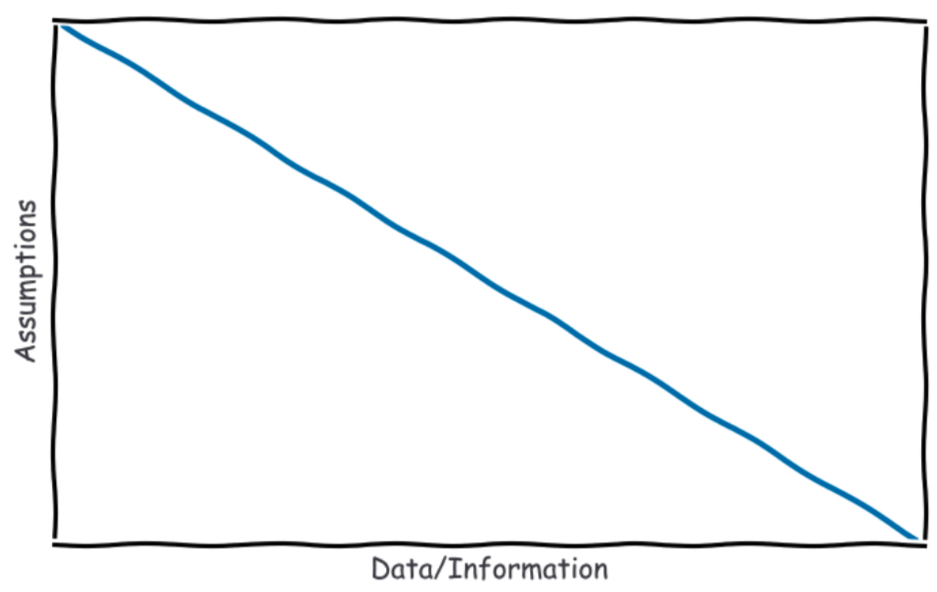
\includegraphics[width=0.7\linewidth]{images/phd/pareto.png}
\caption{The pareto frontier of an optimal model. Inspired by Carl Henrik. }
\end{figure}
\end{frame}


\begin{frame}{Tropical cyclones are heat engines}
\begin{figure}

\includegraphics[width=0.8\linewidth]{images/phd/drawing232115.png}
\caption{Theory from \cite{emanuel1986air}. }
\end{figure}
\end{frame}


\begin{frame}{Tropical cyclones are heat engines}

\vspace{-20pt}
\begin{figure}
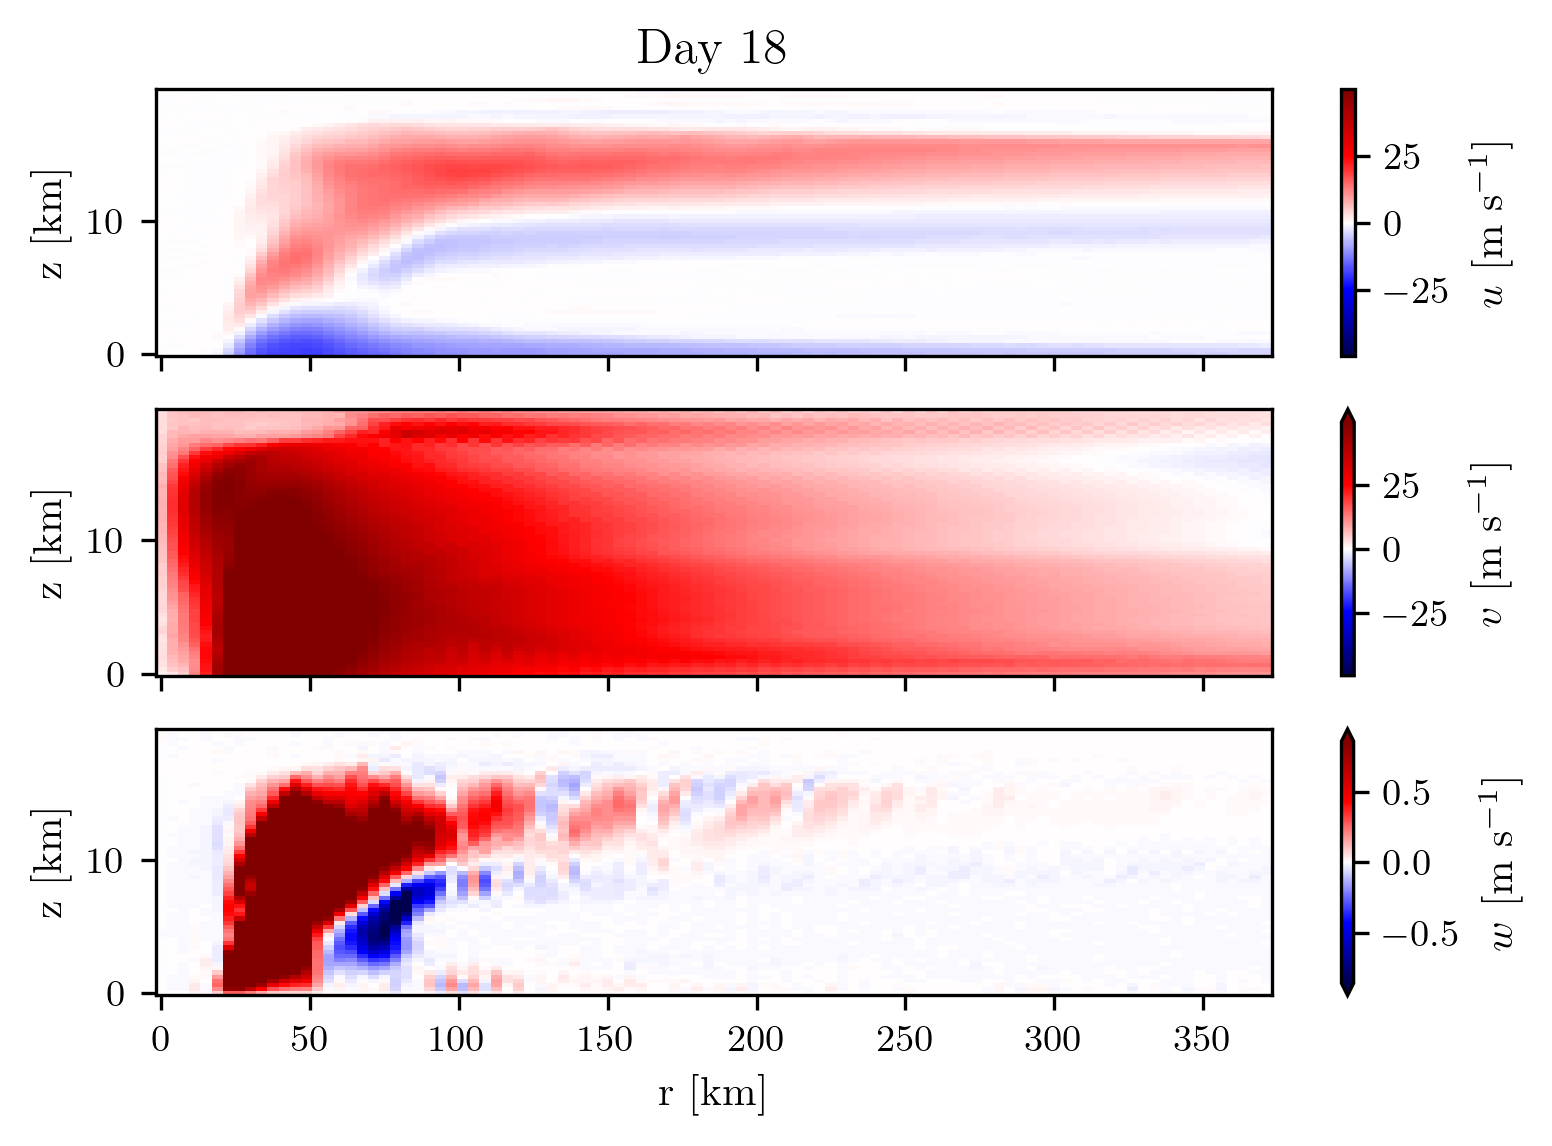
\includegraphics[width=0.7\linewidth]{images/phd/rot-day18.png}
\caption{Azimuthally symetric model from \cite{Rotunno1987AnNumerical}. }
\end{figure}
\end{frame}

\begin{frame}{Katrina was powered by heat sucked out of the Gulf of Mexico}
    \vspace{-40pt}
    \centering

    \begin{figure}
    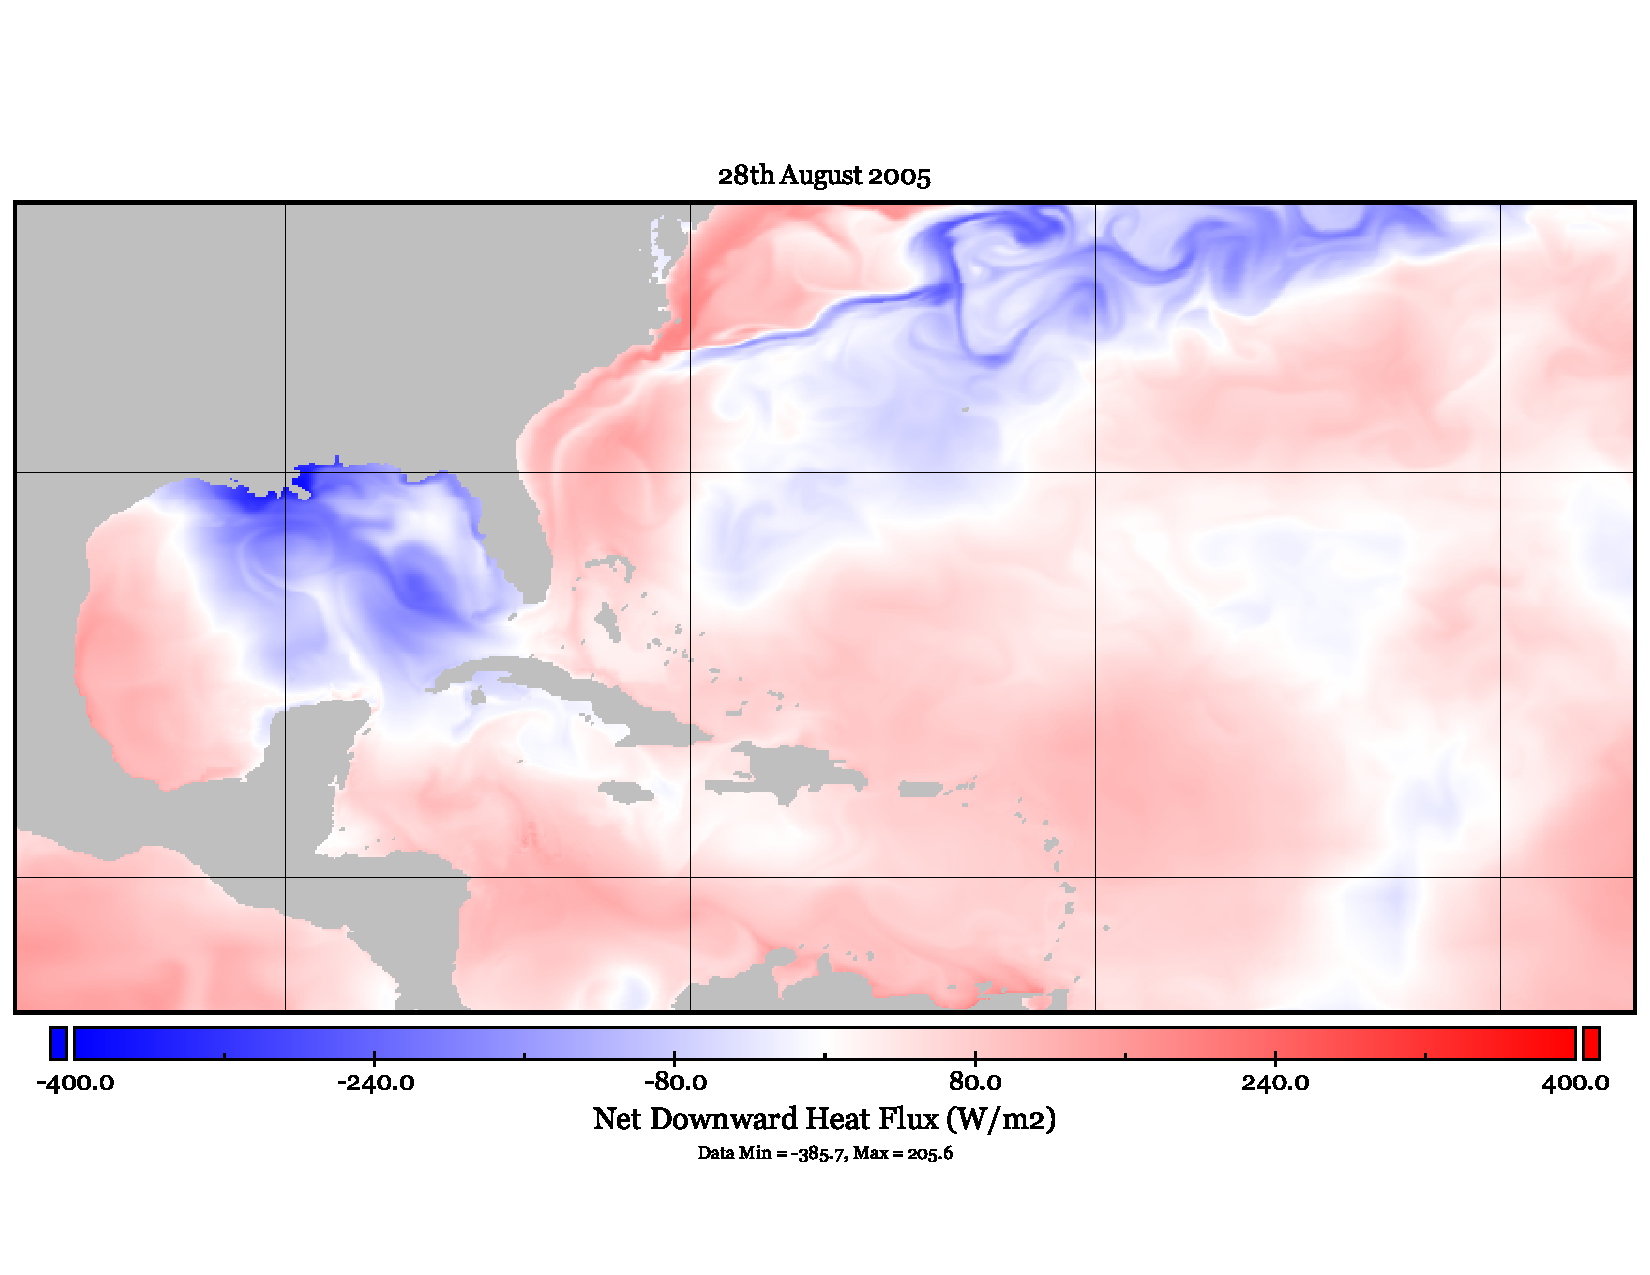
\includegraphics[width=0.75\linewidth]{kat-heat.pdf}\vspace{-30pt}
    \caption{ Daily downwards heat flux as Katrina hit from ORAS12 model forced by ERA5 (Met Office)}
    \end{figure}

\end{frame}

\begin{frame}{Storm surges are the most deadly aspect of tropical cyclones}
\begin{figure}
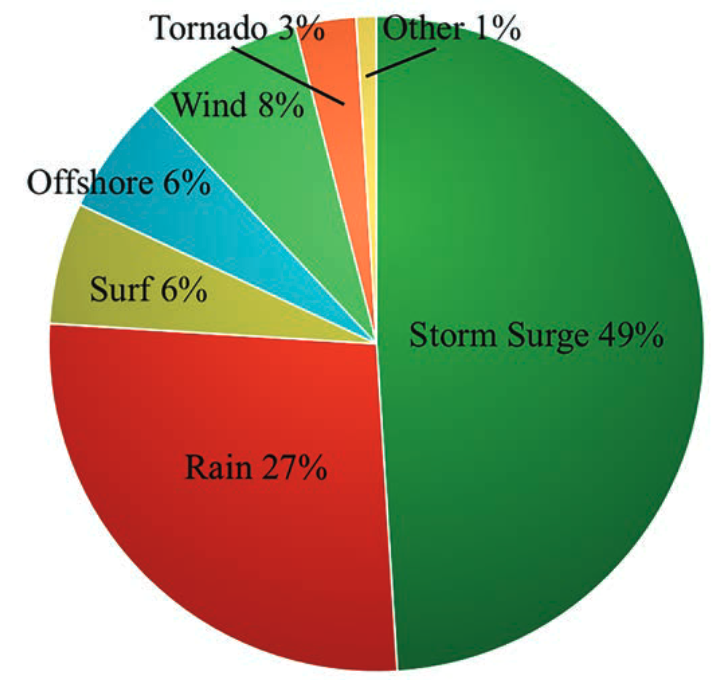
\includegraphics[width=0.5\linewidth]{images/phd/talea_breakdown.png}
\caption{Cause of death breakdown from severe TC in US from \cite{Mayo2019PredictingResilience}. }
\end{figure}
\end{frame}


\begin{frame}{Improving a classical statistical model
    with physics
    (3-6 months)}
    
    \vspace{100pt}

    \begin{itemize}
        \item \cite{Chavas2013U.S.Perspective} showed that physical covariates could be used to improve an extreme value theory model. 
        \begin{itemize}
            \item $V_{\mathrm{max}}$
            \item Slope to 30m isobath
        \end{itemize}
        
        \item Can improve the physical covariates to improve the fit:
        \begin{itemize}
            \item $P_{\mathrm{central}}$ (\cite{Chavas2017PhysicalRelationship})
            \item Responsiveness measure from MSci project.
        \end{itemize}
    \end{itemize}
\end{frame}

\begin{frame}{How can we cheapen a model? (emulation) (6-9 months)}

    \vspace{105pt}

\begin{itemize}
    \item ADCIRC/SWAN model emulated with:
    \begin{itemize}
        \item Neural network type model (e.g.~Rachel Furner's work)
        \item Physics approximation (as per MRes).
        \item Hybrid neural network (e.g.~\cite{beucler2019achieving})
        \begin{itemize}
            \item Penalisation of physics breaking or physics constraints.
        \end{itemize}
    \end{itemize}
    \item  Fair playing field to see which method is best for accuracy/cost.
\end{itemize}
\end{frame}

\begin{frame}{Can we reliably downscale in historical period? (9 months)}

    \vspace{120pt}
\Large
\begin{itemize}
    \item Input: ECMWF reanalysis.
    \item Target: East US tidal gauges.
    \item Model: winner/winners of emulation task.
\end{itemize}
\end{frame}

\begin{frame}{Can this downscaling be used with CMIP6? (9 months)}

    \vspace{120pt}
\Large
    \begin{itemize}
    \item Input: CMIP6 ensemble members.
    \item Output: Surge heights at coast.
    \item Model: Verified algorithm from historical period.
    \item Bias correction: e.g. adding indices like NINO3.4 as physical covariates extreme value model.
    \end{itemize}
\end{frame}

\begin{frame}{Conclusion}
\Large
    \begin{itemize}
        \item Aim: to incorporate more physical knowledge into statistical and
         machine learning methods in order to improve our ability to
          predict tropical cyclone storm surge hazard
        \item Schedule:
    \begin{itemize}
        \item Classical statistics (3-6 months).
        \item Emulation of ADCIRC/SWAN (6-9 months).
        \item Downscaling from ECMWF to tidal gauges (9 months).
        \item Downscaling from CMIP6 (with bias correction) (9 months).
        \item Write up (6 months).
    \end{itemize}

\end{itemize}

\end{frame}


